\newpage
\section{Design Considerations}

\subsection*{Architecture}

Figure~\ref{fig:architecture-diagram} shows the architecture of this application:

\begin{figure}[ht]
  \centering
  \includegraphics*[width=\textwidth]{assets/images/diagrams/architecture-diagram.png}
  \caption{Architecture of the application}
  \label{fig:architecture-diagram}
\end{figure}

\subsection*{Sequence Diagram}

Figure~\ref{fig:sequence-diagram}, shows the main interactions between actors in the application.

\begin{figure}[ht]
  \centering
  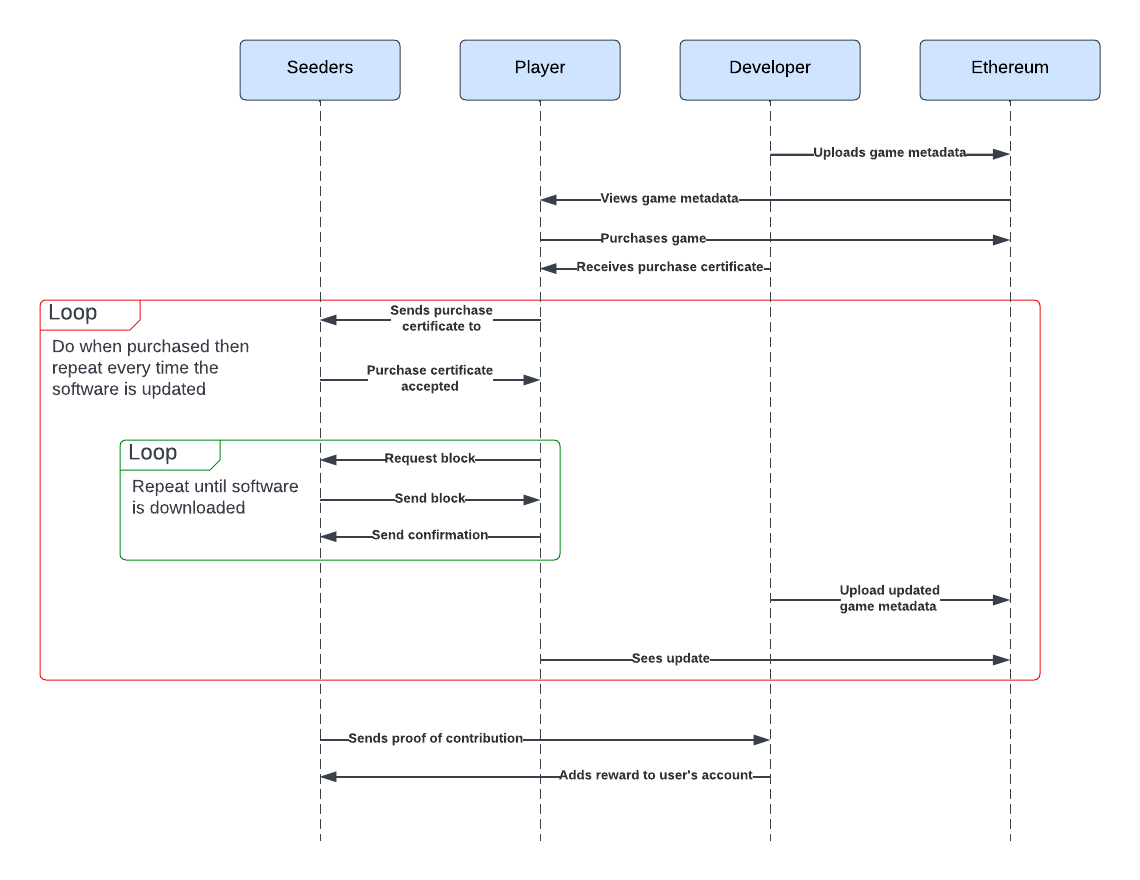
\includegraphics[width=.95\textwidth]{assets/images/diagrams/seqeunce-diagram.png}
  \caption{A sequence diagram showing some of the main interactions within this application}
  \label{fig:sequence-diagram}
\end{figure}


\subsection{On-Chain}

\subsubsection*{Type of Blockchain}

To satisfy \textbf{NF\_M1} and \textbf{NF\_M2}, we will need to use a public blockchain, which will benefit our project by:
\vspace{2mm}
\begin{itemize}
  \item being accessible to a larger user-base, which should boost availability and scalability (\textbf{NF\_S1}),
  \item reducing the risk of censorship (\textbf{NF\_M1}), and
  \item providing greater data integrity (\textbf{NF\_M4})
\end{itemize}

\vspace{2mm}\noindent Ethereum is a public blockchain that allows developers to publish their own distributed applications to it. It comes with an extensive development toolchain so is an obvious choice for this project (\textbf{F\_M8}).

\subsubsection*{Data}

Ideally, we want to store a minimal amount of data on the blockchain as possible such that any user can easily identify and download games that have been uploaded. As games are typically very large data objects it is an important aspect of this project to present an isomorphism between the real data and what we actually store on the blockchain. This project will break each file, in each game, down into constant-sized chunks and will store the hashes of each shard on the blockchain. This massively reduces the amount of data we will need to store but will still allow users to trust the data that they download.
\x
For each game, we will store:

\begin{itemize}
  \item The hash data presented as a tree that maps to the directory structure of the uploaded game (see Figure~\ref{fig:hash-storage}),
  \item Information about the game, including its title, version, release date, developer, and a reference to a previous version if it exists.
\end{itemize}

\subsection*{Purchasing Content}

Users will purchase content from sellers using Ether (\textbf{F\_M9}) and will be provided with a proof of purchase (\textbf{F\_M10}) that is encrypted with the developer's private key. By using public key infrastructure, it gives proof of purchases authenticity that allows them to be validated by any node in the network.
\x
The proof of purchase will include: the root hash of the title purchased, the seller's address, the buyer's address, a timestamp, and a unique seeder token to be used for proving distribution.

\subsection{Off-Chain}

\subsubsection*{Uploading Content}
\label{subsec:upload-content}

For developers to upload their game (\textbf{F\_M5}), they must provide a digital certificate to prove their identity (\textbf{NF\_M3}) as well as the required metadata (\textbf{F\_M1}) for identifying, downloading and verifying their game.
The developer is then expected to allow users to purchase the game off them and seed the game to at least an initial group of users.

\begin{figure}[ht]
  \centering
  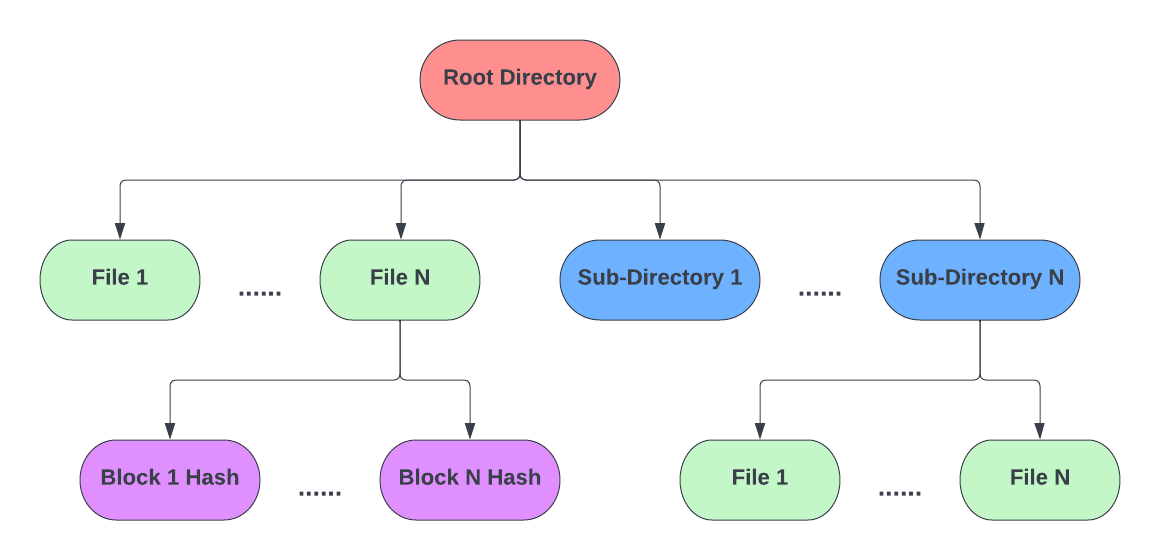
\includegraphics[width=.85\textwidth]{assets/images/diagrams/block-body.png}
  \caption{Hash data about shards will be stored in a tree that mimics the folder structure of the data}
  \label{fig:hash-storage}
\end{figure}

\subsection*{Downloading Content}

Games will be content addressable, using their root hash stored on the blockchain. This will be used to help connect nodes who are interested in the same content (\textbf{F\_M3}). Once a user connects to a node it will:
\vspace{2mm}
\begin{enumerate}
  \item Send their proof of purchase (\textbf{F\_S2}).
  \item request individual shards from the node using the shard's hash (\textbf{F\_M2}),
  \item use the metadata from the blockchain to verify the shard's contents (\textbf{F\_M7}),
  \item send a confirmation message that proves the successful transfer of a block (\textbf{F\_S1}),
  \item and repeat this until the entirety of the game is installed (\textbf{F\_M6}).
\end{enumerate}

\vspace{2mm}\noindent As the blockchain will only be used to store metadata about games uploaded to the network, not every node will have each game installed. Instead, this project will take ideas from networks like BitTorrent, where nodes will seek out peers who have the game installed using a tracker hosted by the uploader.

\subsection*{Updating Content}

To satisfy \textbf{F\_M4}, developers will perform the same steps as in \textbf{Uploading Content} but will also include the hash of a previous block that contains the older version of the game. This relationship will allow users ownership to all versions of a game they have purchased and not just a singular version. This will include the restriction that only the original uploader can upload an update for their game (\textbf{NF\_S2}).

\vspace{2mm}\noindent Each version will be considered as a standalone game and will require users to download the entirety by scratch. Whilst this isn't reflective of how updates are typically managed, this will be acceptable for the scope of this project and any changes will be considered as a future extension to this project.

\subsubsection*{Downloadable Content}

Developers will typically offer paid or free DLC (\textbf{F\_S3}) for their games that users will purchase separately. Each DLC will need:

\begin{enumerate}
  \item \textbf{Dependency} A reference to the oldest version of the game they apply to, and
  \item \textbf{Previous Version} A pointer to the previous version of the DLC.
\end{enumerate}

\begin{figure}[ht]
  \centering
  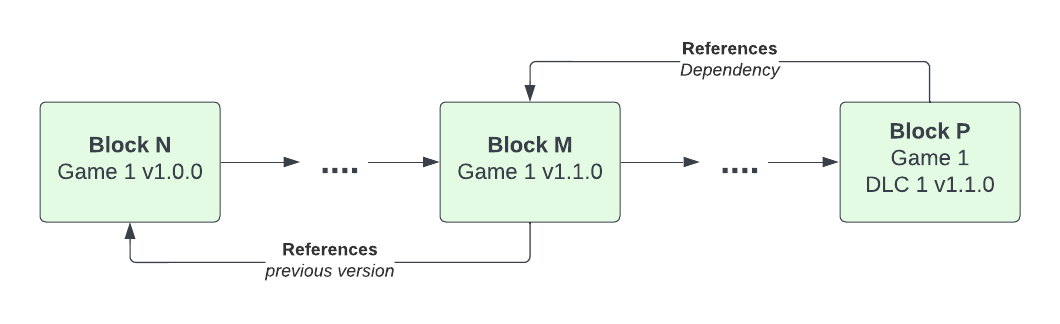
\includegraphics[width=.85\textwidth]{assets/images/diagrams/software.png}
  \caption{How blocks relate to each other. An update will reference the previous version whilst a DLC will reference, which piece of software and version it is dependent on.}
\end{figure}

\subsection*{Proving Contribution}

A purchase certificate will include a confidential \textit{seeder token}. When a user successful downloads a shard of data they will send a confirmation message, including their seeder token, that is encrypted with the game developer's public key. A user will prove their contribution (\textbf{F\_S1}) by sending a collection of these messages to the developer, who can decrypt and validate the tokens.
